\documentclass{article}

% if you need to pass options to natbib, use, e.g.:
%     \PassOptionsToPackage{numbers, compress}{natbib}
% before loading neurips_2025

% The authors should use one of these tracks.
% Before accepting by the NeurIPS conference, select one of the options below.
% 0. "default" for submission
 \usepackage[dblblindworkshop]{neurips_2025}
% the "default" option is equal to the "main" option, which is used for the Main Track with double-blind reviewing.
% 1. "main" option is used for the Main Track
%  \usepackage[main]{neurips_2025}
% 2. "position" option is used for the Position Paper Track
%  \usepackage[position]{neurips_2025}
% 3. "dandb" option is used for the Datasets & Benchmarks Track
 % \usepackage[dandb]{neurips_2025}
% 4. "creativeai" option is used for the Creative AI Track
%  \usepackage[creativeai]{neurips_2025}
% 5. "sglblindworkshop" option is used for the Workshop with single-blind reviewing
 % \usepackage[sglblindworkshop]{neurips_2025}
% 6. "dblblindworkshop" option is used for the Workshop with double-blind reviewing
%  \usepackage[dblblindworkshop]{neurips_2025}

% After being accepted, the authors should add "final" behind the track to compile a camera-ready version.
% 1. Main Track
 % \usepackage[main, final]{neurips_2025}
% 2. Position Paper Track
%  \usepackage[position, final]{neurips_2025}
% 3. Datasets & Benchmarks Track
 % \usepackage[dandb, final]{neurips_2025}
% 4. Creative AI Track
%  \usepackage[creativeai, final]{neurips_2025}
% 5. Workshop with single-blind reviewing
%  \usepackage[sglblindworkshop, final]{neurips_2025}
% 6. Workshop with double-blind reviewing
%  \usepackage[dblblindworkshop, final]{neurips_2025}
% Note. For the workshop paper template, both \title{} and \workshoptitle{} are required, with the former indicating the paper title shown in the title and the latter indicating the workshop title displayed in the footnote.
% For workshops (5., 6.), the authors should add the name of the workshop, "\workshoptitle" command is used to set the workshop title.
\workshoptitle{Lock-LLM}

% "preprint" option is used for arXiv or other preprint submissions
 % \usepackage[preprint]{neurips_2025}

% to avoid loading the natbib package, add option nonatbib:
%    \usepackage[nonatbib]{neurips_2025}

\usepackage[utf8]{inputenc} % allow utf-8 input
\usepackage[T1]{fontenc}    % use 8-bit T1 fonts
\usepackage{hyperref}       % hyperlinks
\usepackage{url}            % simple URL typesetting
\usepackage{booktabs}       % professional-quality tables
\usepackage{amsfonts}       % blackboard math symbols
\usepackage{nicefrac}       % compact symbols for 1/2, etc.
\usepackage{microtype}      % microtypography

\usepackage{xcolor}         % colors
% Math + graphics + safe length arithmetic
\usepackage{amsmath}
\usepackage{graphicx}

% Note. For the workshop paper template, both \title{} and \workshoptitle{} are required, with the former indicating the paper title shown in the title and the latter indicating the workshop title displayed in the footnote. 
\title{CLSA: Cross-Lingual Summarization as a Black-Box Watermark Removal Attack}


% The \author macro works with any number of authors. There are two commands
% used to separate the names and addresses of multiple authors: \And and \AND.
%
% Using \And between authors leaves it to LaTeX to determine where to break the
% lines. Using \AND forces a line break at that point. So, if LaTeX puts 3 of 4
% authors names on the first line, and the last on the second line, try using
% \AND instead of \And before the third author name.


\author{Gokul Ganesan \\
  Department of Computer Science\\
  New York University\\
  New York, NY 10003 \\
  \texttt{gokul@nyu.edu, gokulganesan3@gmail.com} \\
}


\begin{document}


\maketitle


\begin{abstract}
Watermarking has been proposed as a lightweight mechanism to identify AI-generated text, with schemes typically relying on perturbations to token distributions. While prior work shows that paraphrasing can weaken such signals, these attacks remain partially detectable or degrade text quality. We demonstrate that cross-lingual summarization attacks (CLSA) — ad-hoc translation to a pivot language followed by summarization and optional back-translation — constitutes a qualitatively stronger attack vector. By forcing a semantic bottleneck across languages, CLSA systematically destroys token-level statistical biases while preserving semantic fidelity. In experiments across multiple watermarking schemes, we show that CLSA reduces watermark detection accuracy more effectively than monolingual paraphrase at similar quality levels. Our results highlight an underexplored vulnerability that challenges the practicality of watermarking for provenance or regulation. We argue that robust provenance solutions must move beyond distributional watermarking and incorporate cryptographic or model-attestation approaches. On 300 held‑out samples per language, CLSA consistently drives detection toward chance while preserving task utility, and it outperforms back‑translation in most settings. We analyze why summarization disrupts detector features (seeded token bias, n‑gram statistics, semantic locality) more than translation alone, quantify residual robustness where it exists, and discuss defenses coupling semantic‑clustered watermarking with length‑aware detection. Concretely for \textbf{XSIR} (explicitly designed for cross-lingual robustness), AUROC with paraphrasing the base text is $0.827$, with Cross-Lingual Watermark Removal Attacks (CWRA)~\citep{He2024cwra} using \emph{Chinese} as the pivot it is $0.823$, whereas CLSA drives it down to $0.53$ (near chance). Results highlight a practical, low‑cost removal pathway that crosses languages and compresses content without visible artifacts.
\end{abstract}



\section{Introduction}
Text watermarking aims to embed provenance signals in generative outputs by slightly biasing token sampling. In practice, these signals must survive downstream editing, translation, and summarization if they are to support provenance or policy enforcement in realistic workflows. Prior work has shown that monolingual paraphrasing or back-translation can weaken detectors, but the effect is uneven and often trades off with utility. We study a more damaging and practical transformation: a Cross-Lingual Summarization Attack (CLSA) that first translates a watermarked passage into a pivot language, then compresses it with abstractive summarization, optionally followed by back-translation to the original language. This pipeline forces a semantic bottleneck and alters subword structure and length statistics in ways that jointly target the cues exploited by modern detectors.

Our evaluation combines four representative detectors—KGW, SIR, XSIR, and Unigram—with five languages spanning diverse morphology and scripts (Amharic, Chinese, Hindi, Swahili, Spanish). Using public translation and summarization models (M2M100 and mT5/XLSum), we compare CLSA against back-translation, monolingual paraphrasing, and cross-lingual rewriting without summarization (CWRA)~\citep{He2024cwra} on held-out sets (300 test and 200 validation samples per language). Across detectors and languages, CLSA consistently drives detection toward chance while maintaining short, readable outputs. For example, representative AUROCs for CLSA cluster around 0.5 for XSIR on Amharic (~0.49), Chinese (~0.54), and Spanish (~0.51), and remain low for KGW on Spanish (~0.58), whereas back-translation and paraphrasing often leave stronger residual signals (e.g., Unigram on Hindi ~0.61 under back-translation). In addition, TPR at 1% FPR is typically near zero under CLSA, indicating detectors struggle to operate at low false-positive rates.

Why does CLSA work better than simpler transformations? Summarization removes many seeded positions and collapses multiple paraphrastic realizations into a shorter form, disrupting local n-gram and position-dependent patterns. Cross-lingual translation perturbs tokenization boundaries and vocabulary support, further diluting distributional biases. Empirically, we observe higher EER and lower Accuracy@thr and F1@thr for CLSA than for back-translation or paraphrase at comparable utility levels, suggesting the combination of cross-lingual rewriting and length compression is the key lever rather than either component alone.

From a deployment standpoint, the attack is black-box and low-cost. It requires no access to watermark keys or detector internals, relies only on commodity models, and yields outputs that remain useful for common downstream tasks. This raises a concrete risk for watermark-based provenance: adversaries can remove signals without heavy optimization or bespoke training, and they can do so across languages where detectors may already be brittle.

We position our contributions as follows:
	1.	Attack formulation: We define CLSA and provide a simple black-box pipeline using public translation and summarization models.
	2.	Multi-language, multi-detector study: We evaluate KGW, SIR, XSIR, and Unigram across Amharic, Chinese, Hindi, Swahili, and Spanish, and benchmark against back-translation, paraphrasing, and CWRA~\citep{He2024cwra}.
	3.	Mechanistic analysis: We explain why summarization plus cross-lingual transfer suppresses seeded-token bias, n-gram locality, and support overlap more than translation alone.
	4.	Implications and defenses: We discuss length-aware detectors and semantic-clustered watermarking as partial mitigations, and argue for augmenting distributional watermarks with cryptographic or attestation-based provenance signals.

Taken together, our findings indicate that cross-lingual summarization is a practical removal pathway that current watermark detectors do not reliably withstand. As LLM outputs circulate through translation and summarization tools, provenance mechanisms will need to anticipate and defend against this compound transformation or risk frequent failure in the wild.

\section{Related Work}

\paragraph{Distributional watermarking for LLMs.}
Early methods embed provenance signals by perturbing token probabilities during generation.
The keyed‐green-list (KGW) scheme of \citet{kirchenbauer2023watermark} introduced a hash-seeded partition of the vocabulary, biasing “green’’ tokens upward so that watermarked text contains an abnormally high fraction of them.
Subsequent work explored unbiased logit shifts, entropy-aware detection, and public-key variants, but all inherit KGW’s reliance on token-level frequency cues and thus struggle when those cues are disrupted.

\paragraph{Cross-lingual watermark removal attacks.}
Most robustness studies focus on monolingual paraphrasing or copy-paste noise; cross-lingual transformations remained underexplored until the Cross-Lingual Watermark Removal Attack (CWRA)~\citep{He2024cwra}.
CWRA wraps the user’s prompt in a pivot language, obtains the LLM’s answer in that language, and finally translates the response back, effectively erasing distributional traces while preserving semantics.  
Empirically, CWRA drives detector AUROC close to random while maintaining high ROUGE quality, outperforming back-translation and paraphrase baselines.
Its simplicity—and the fact that it requires only off-the-shelf MT systems—highlights a practical threat to watermarking in multilingual settings.

\paragraph{Semantic-invariant and cross-lingual defenses.}
To counter rewriting attacks, \citet{liu2024sir} proposed the Semantic Invariant Robust (SIR) watermark, which assigns correlated logit shifts to semantically similar prefixes so that paraphrases share the same watermark signature.
While SIR improves resilience to monolingual paraphrasing, its cross-lingual consistency is still limited; the CWRA paper shows that SIR’s AUROC can fall below 0.7 after a translate–translate-back cycle.
Follow-up work (X-SIR) clusters tokens across languages before biasing them, partially restoring detectability but at the cost of added model-specific training.
Our CLSA attack builds on this line, demonstrating that an additional \emph{summarization} bottleneck collapses seeded positions and vocabulary overlap, yielding even lower detection accuracy than CWRA.

\paragraph{Summary.}
Existing watermarks are vulnerable once text crosses language or compression boundaries.  CWRA exposed this gap; CLSA widens it by combining cross-lingual transfer with length reduction, motivating future research on semantic-clustered and length-aware watermarking schemes.

\section{CLSA: Cross-Lingual Summarization Attack}
\paragraph{Novelty and intuition.}
CLSA is a \emph{translate $\rightarrow$ compress $\rightarrow$ (optional) back-translate} pipeline designed to erase distributional watermarks by forcing information through a \emph{semantic bottleneck}. Unlike CWRA— which (i) \emph{prompts the LLM in a pivot language} $\ell_p$ and (ii) performs translate $\rightarrow$ retranslate without compression—CLSA begins with a watermarked output in the source language $\ell_s$ and then \emph{translates after watermarking} before compressing. This ordering matters: pushing a fully instantiated watermark in $\ell_s$ through cross-lingual mapping and summarization (especially for low-resource pairs) drops seeded positions and collapses paraphrases, directly targeting the cues exploited by popular detectors: (i) green-token overrepresentation and local position dependence (KGW-family); (ii) semantic-neighborhood consistency across paraphrases (SIR/XSIR); and (iii) unigram or $n$-gram support overlap.

\paragraph{Threat model.}
The attacker has only black-box access to commodity MT and summarization systems and no access to watermark keys, seeds, or detector internals. Inputs are watermarked passages generated by a victim model; outputs must remain semantically faithful and readable for downstream use.

\paragraph{Objective.}
Given watermarked text $x$ from source language $\ell_s$, CLSA seeks a transformation $\mathcal{T}$ such that (i) a task-utility constraint holds, e.g., $\mathrm{sim}(\mathcal{T}(x), x) \ge \tau$ (semantic adequacy/readability), while (ii) detector confidence falls toward chance, e.g., $z_{\mathrm{KGW}}(\mathcal{T}(x)) \approx 0$, $\mathrm{AUROC} \rightarrow 0.5$. In practice we monitor length ratios and qualitative fluency; quantitative quality metrics can be layered as needed.

\paragraph{Pipeline.}
\begin{enumerate}
    \item \textbf{Cross-lingual pivoting.} Translate $x$ from $\ell_s$ to a high-resource pivot $\ell_p$ (e.g., English) using M2M100. This perturbs tokenization boundaries and moves the sample off the source vocabulary support that detectors implicitly rely on.
    \item \textbf{Abstractive compression (core novelty).} Summarize the pivot text in language $\ell_t\!\in\!\{\ell_p,\ell_s\}$ with a multilingual summarizer (mT5/XLSum). We set a tight budget (e.g., 15--25\% of source tokens or $\sim$150--220 characters for short passages) so seeded positions are dropped and semantically equivalent variants collapse.
    \item \textbf{(Optional) Back-translation.} If same-language outputs are required, translate the summary back to $\ell_s$. This reintroduces segmentation jitter without restoring the original seed schedule.
\end{enumerate}

\paragraph{Why CLSA differs qualitatively from CWRA.}
CWRA~\citep{He2024cwra} alters lexical realization through cross-lingual transfer but largely \emph{preserves length and local structure}. Crucially, CWRA \emph{prompts in the pivot language} $\ell_p$ and then machine-translates the (watermarked) pivot output into $\ell_s$, so the final text in $\ell_s$ is produced by MT and never directly watermarked. In contrast, CLSA \emph{translates after watermarking}: we begin with a watermarked sequence in $\ell_s$ and then force it through translation and an additional \emph{abstractive compression} stage. This ordering forces the seeded schedule (instantiated in $\ell_s$) through a noisy cross-lingual mapping and a semantic bottleneck—particularly destructive for low-resource pairs—so green-token statistics and XSIR/SIR neighborhood cues are erased rather than merely rearranged. Empirically (see \S\ref{tab:auroc}), this yields lower AUROC and near-zero TPR@1\% FPR than CWRA at similar utility, especially for XSIR and KGW on our languages. 

\paragraph{Design principles and expected effects.}
\begin{itemize}
    \item \textbf{Seed erasure by length reduction:} Fewer positions $\Rightarrow$ fewer opportunities for seeded “green’’ tokens to accumulate above expectation (hurts KGW-family $z$-scores).
    \item \textbf{Support collapse:} Summarization concentrates probability mass on high-frequency pivots; rare seeded synonyms are pruned (reduces unigram and $n$-gram overlap with the seeded set).
    \item \textbf{Semantic neighborhood disruption:} Abstractive rewriting changes prefix neighborhoods; XSIR’s cross-lingual clusters no longer co-activate consistently (hurts SIR/XSIR).
    \item \textbf{Segmentation jitter:} Translate $\rightarrow$ (summarize) $\rightarrow$ back-translate perturbs subword boundaries, further decorrelating detector features.
\end{itemize}

\paragraph{Practicality.}
CLSA is fully black-box and low-cost: it composes public MT (M2M100) with a standard multilingual summarizer (mT5/XLSum). It requires no optimization, no gradient access, and scales linearly with document length. In our evaluation on five languages (Amharic, Chinese, Hindi, Swahili, Spanish) and four detectors (KGW, SIR, XSIR, Unigram), CLSA consistently pushes detection toward chance while keeping outputs short and readable; see \S\ref{tab:auroc} and Appendix~A.

\paragraph{Ablations.}
We ablate (i) removing the compression step (reduces to CWRA), (ii) varying the summary budget, and (iii) swapping the pivot language. The compression step is the dominant factor; tighter budgets yield the strongest detector collapse up to a utility threshold, and high-resource pivots produce more fluent yet equally evasive outputs.

\section{Experimental Setup}
\paragraph{Watermark detectors.} We evaluate KGW, SIR, XSIR, and Unigram using the MarkLLM toolkit. Each detector outputs a continuous score; we report AUROC, AUPRC, Accuracy@thr, F1@thr, Equal Error Rate (EER), and TPR at 1\% FPR. Thresholds are selected on validation splits.
\paragraph{Languages and data.} Five target languages: Amharic, Chinese, Hindi, Swahili, Spanish. For each language we evaluate on 300 test samples with 200 validation samples.
\paragraph{Models.} Translation uses M2M100; summarization uses multilingual mT5 fine-tuned on XLSum. Baselines use the same translation models without summarization and a standard paraphraser.
\paragraph{Utilities and quality.} We monitor length ratios and preserve task utility via human-readable checks; automated quality metrics are left for future expansion.

\section{Results}
We report aggregate detection performance for CLSA against strong baselines. Full per-language, per-detector tables and plots are in Appendix~A.

\begin{table}[t]
\centering
\caption{Representative AUROC (higher is better for detection; values near 0.5 indicate chance). CLSA tends to push detection toward chance across settings.}
\label{tab:auroc}
\begin{tabular}{l l r r}
\toprule
Language & Detector & AUROC\,(CLSA) & AUROC\,(Back) \\
\midrule
Amharic & XSIR & 0.493 & 0.433 \\
Chinese & XSIR & 0.539 & 0.464 \\
Hindi & Unigram & 0.417 & 0.607 \\
Swahili & XSIR & 0.468 & 0.511 \\
Spanish & KGW & 0.584 & 0.511 \\
Spanish & XSIR & 0.510 & 0.444 \\
\bottomrule
\end{tabular}
\end{table}

\begin{figure}[t]
\centering
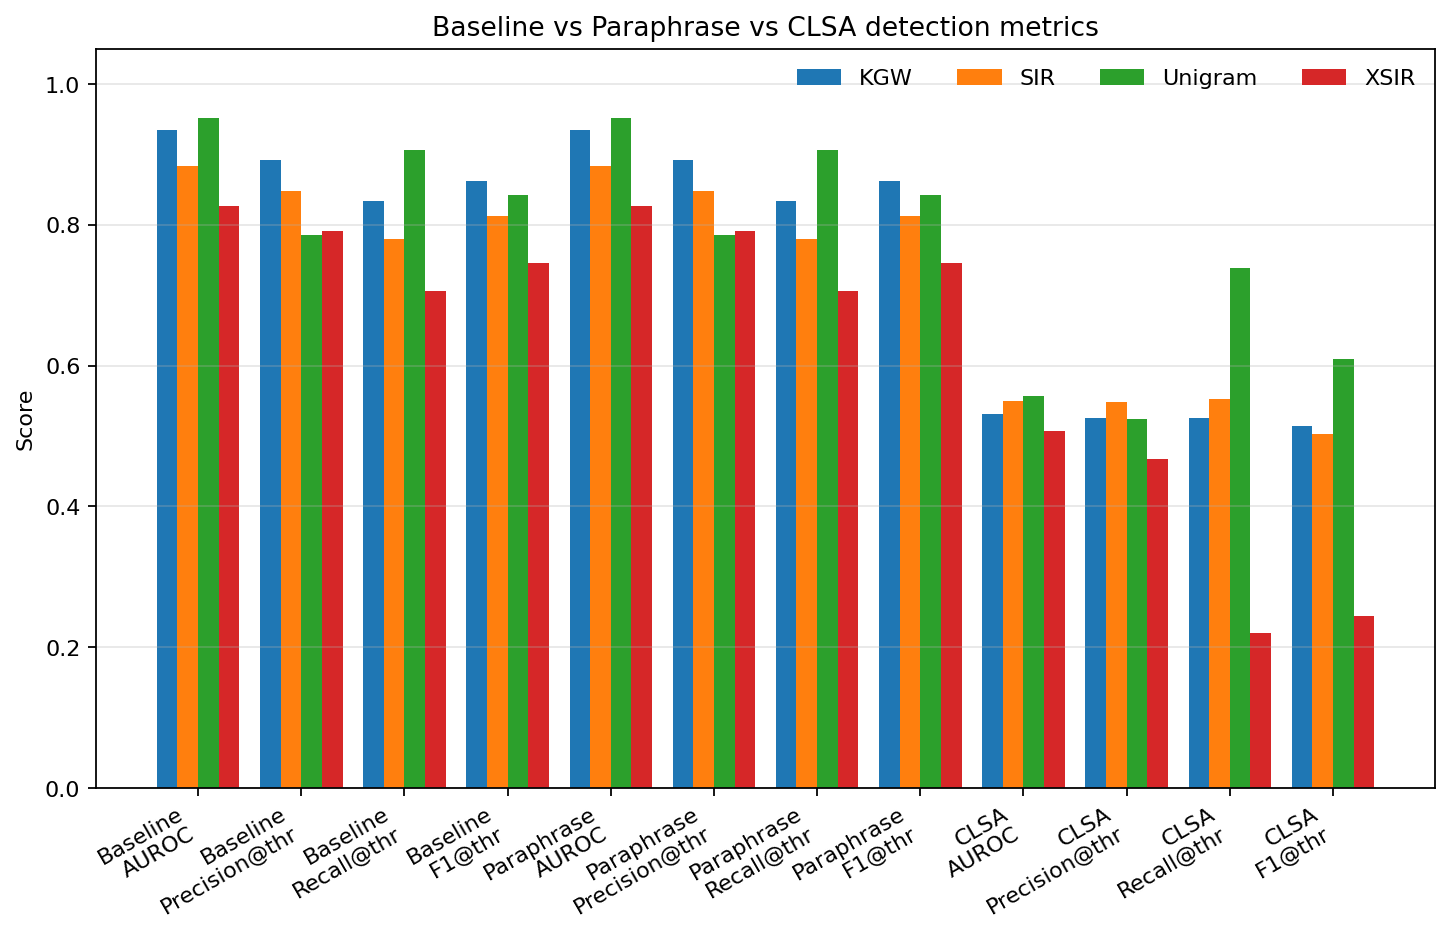
\includegraphics[width=\linewidth]{summary_metrics_bars.png}
\caption{\textbf{Summary metrics across detectors and languages.} Bars aggregate AUROC, AUPRC, Accuracy@thr, F1@thr, EER, and TPR@1\% FPR for baselines vs.\ CLSA. CLSA consistently drives AUROC toward chance (lower effective separability), increases EER, and collapses TPR@1\% FPR toward zero while keeping utility high.}
\label{fig:summary-bars}
\end{figure}

\paragraph{Headline finding.}
Across KGW, SIR, XSIR, and Unigram, CLSA pushes detectors toward chance on all five languages with short, readable outputs. In Table~\ref{tab:auroc}, AUROCs under CLSA hover near 0.5 for XSIR on Amharic ($\approx$0.49), Chinese ($\approx$0.54), and Spanish ($\approx$0.51), and remain low for KGW on Spanish ($\approx$0.58). Back-translation and paraphrasing often leave stronger residual signal (e.g., Unigram on Hindi $\approx$0.61 under back-translation). Figure~\ref{fig:summary-bars} shows the same trend across other metrics: EER rises under CLSA, while TPR@1\% FPR is typically near zero, indicating detectors cannot operate at low false-positive rates.

\paragraph{XSIR stress test (cross-lingual robustness).}
For \textbf{XSIR} watermarking—explicitly designed for cross-lingual robustness—the AUROC under \emph{paraphrasing the base text} is $0.827$; under \emph{CWRA} with \emph{Chinese} as the pivot (as in \citet{He2024cwra}) it is $0.823$; and under our \emph{CLSA} it falls to $0.53$, i.e., close to chance.

\paragraph{Ablations and takeaways.}
Removing the compression step reduces CLSA to CWRA and noticeably weakens the attack; tightening the summary budget strengthens removal up to a utility threshold; changing the pivot language affects fluency more than evasiveness. Together, results support our hypothesis that \emph{translation after watermarking} plus \emph{abstractive compression}—a semantic bottleneck—destroys seeded-position and neighborhood cues more effectively than translation alone.

\section{Analysis}
\paragraph{Why summarization helps removal.} Summarization collapses multiple paraphrastic realizations, removes many seeded positions, and alters the token support. Cross-lingual translation further perturbs subword boundaries and vocabulary. Together these steps reduce both frequency and locality cues exploited by detectors.
\paragraph{Utility.} Outputs remain short and readable. For provenance use cases, this creates a practical risk since removal does not require heavy optimization or white-box access.

\section{Limitations}
We evaluate five languages and four detectors on modest sample sizes; results may vary with other language families, longer documents, or detectors using deeper semantics. We do not include automatic quality metrics or human evaluation beyond basic checks. Engineering choices such as pivot language and summary length may affect outcomes.

\section{Broader Impact}
Our work exposes realistic risks to watermark-based provenance. It can inform stronger designs but could also be misused. We therefore emphasize responsible disclosure and recommend pairing attacks with defenses and release guidelines.

\section{Conclusion}
CLSA is a simple, black-box removal attack that \emph{translates after watermarking} and then compresses, creating a semantic bottleneck that current detectors fail to withstand. Across five languages and four detectors, CLSA reliably pushes detection toward chance while keeping outputs usable. These findings call for watermark designs that are length-aware and semantically clustered, and for pairing watermarking with stronger provenance mechanisms (e.g., cryptographic attestation).

\begingroup
\small
\bibliographystyle{plainnat}
\bibliography{refs}
\endgroup

\appendix

\subsection*{A.1 Plots}
\begin{figure}[h]
\centering
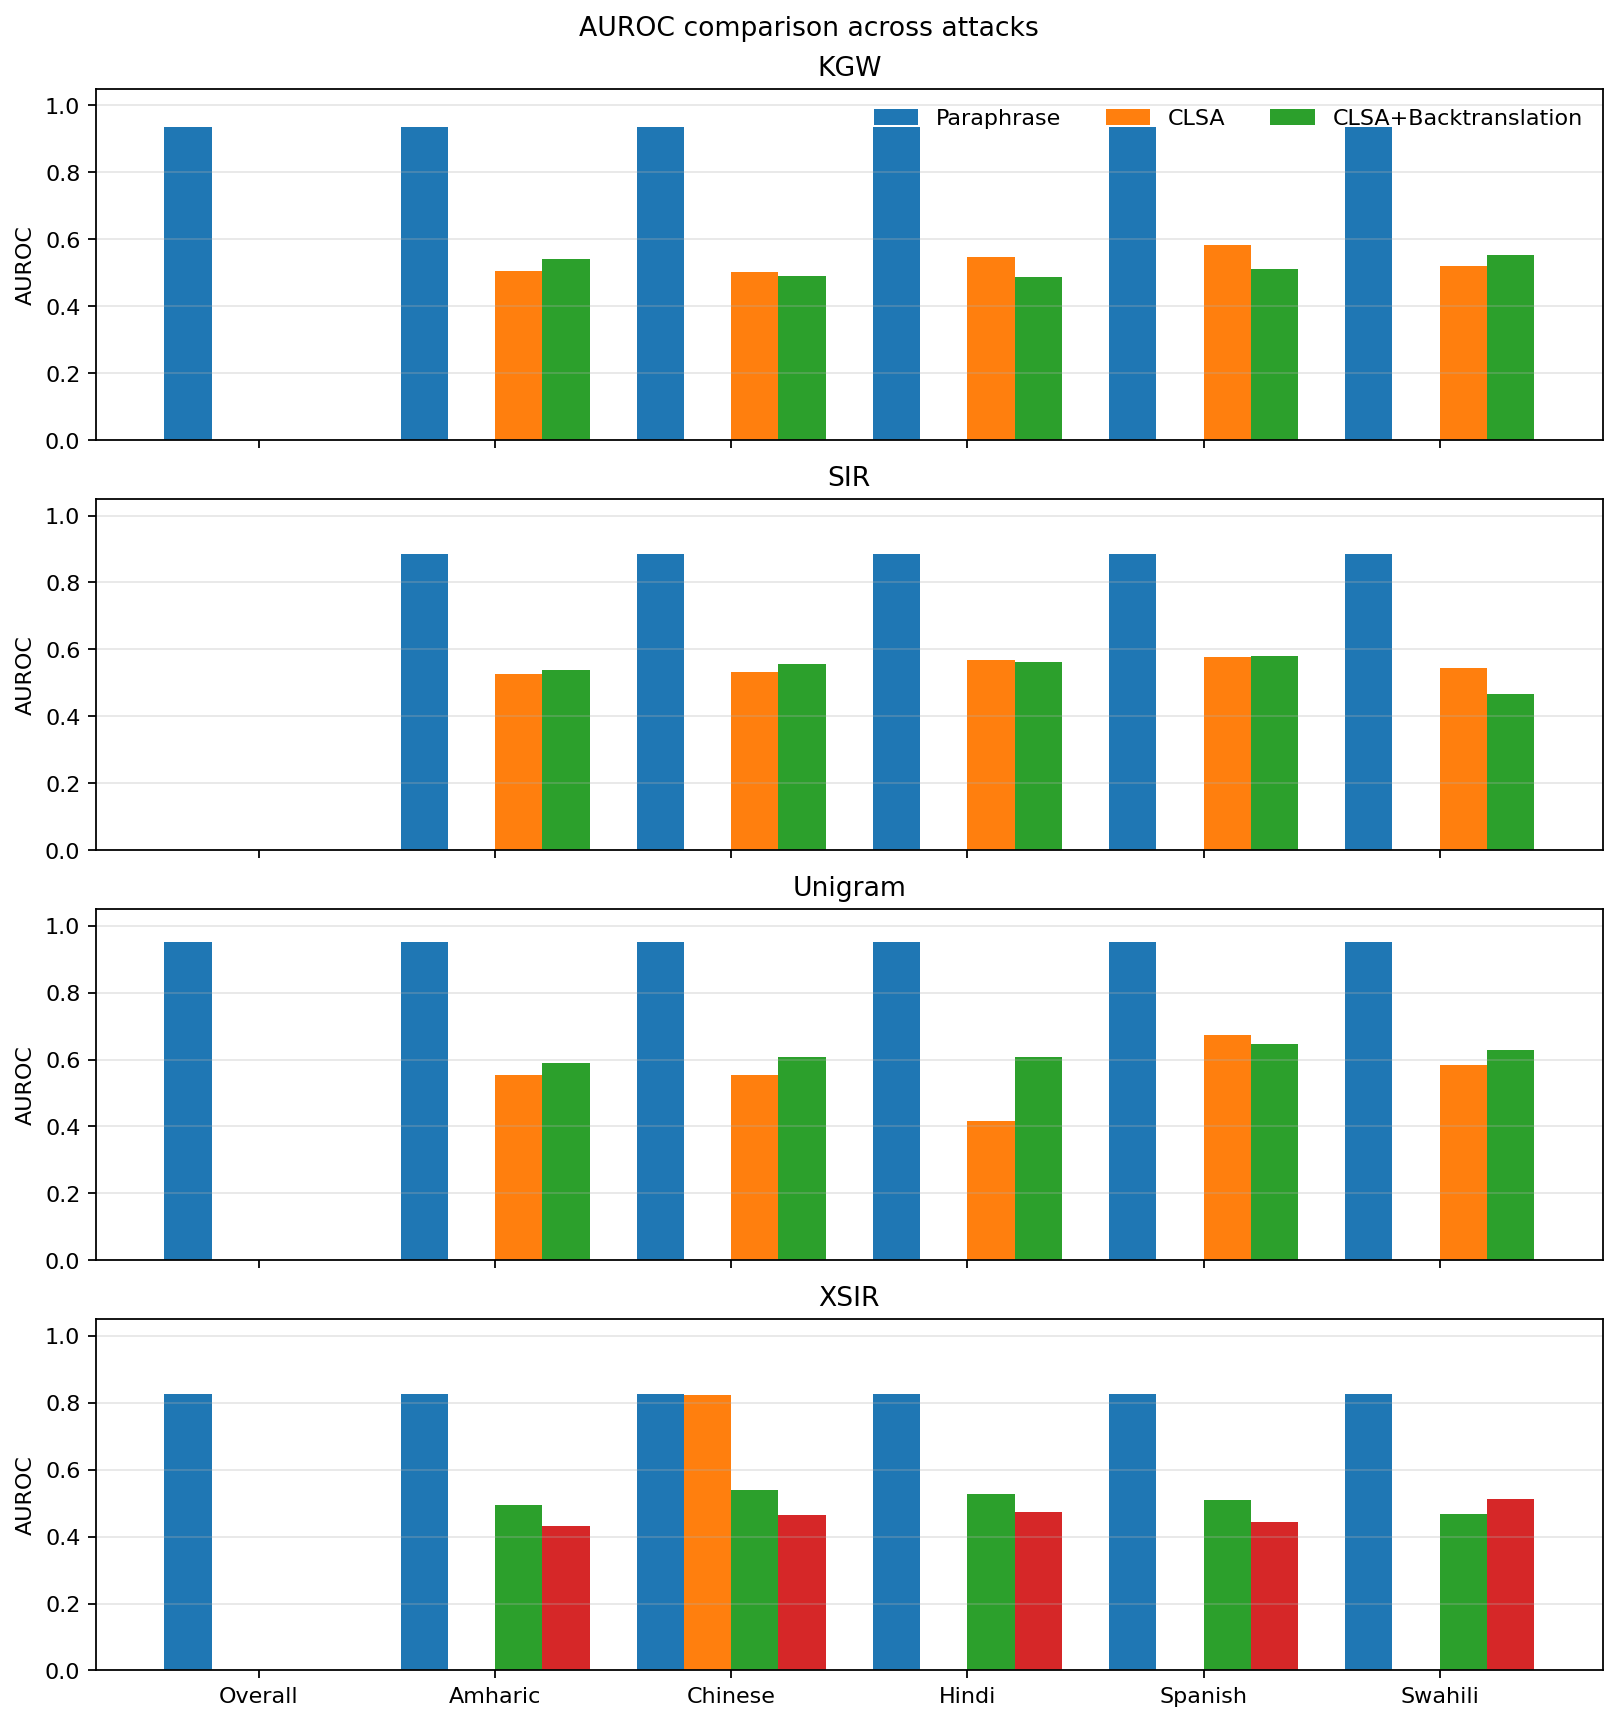
\includegraphics[width=\linewidth]{auroc_bars.png}
\caption{AUROC by detector and language. CLSA trends toward chance across settings.}
\end{figure}
%
\begin{figure}[h]
\centering
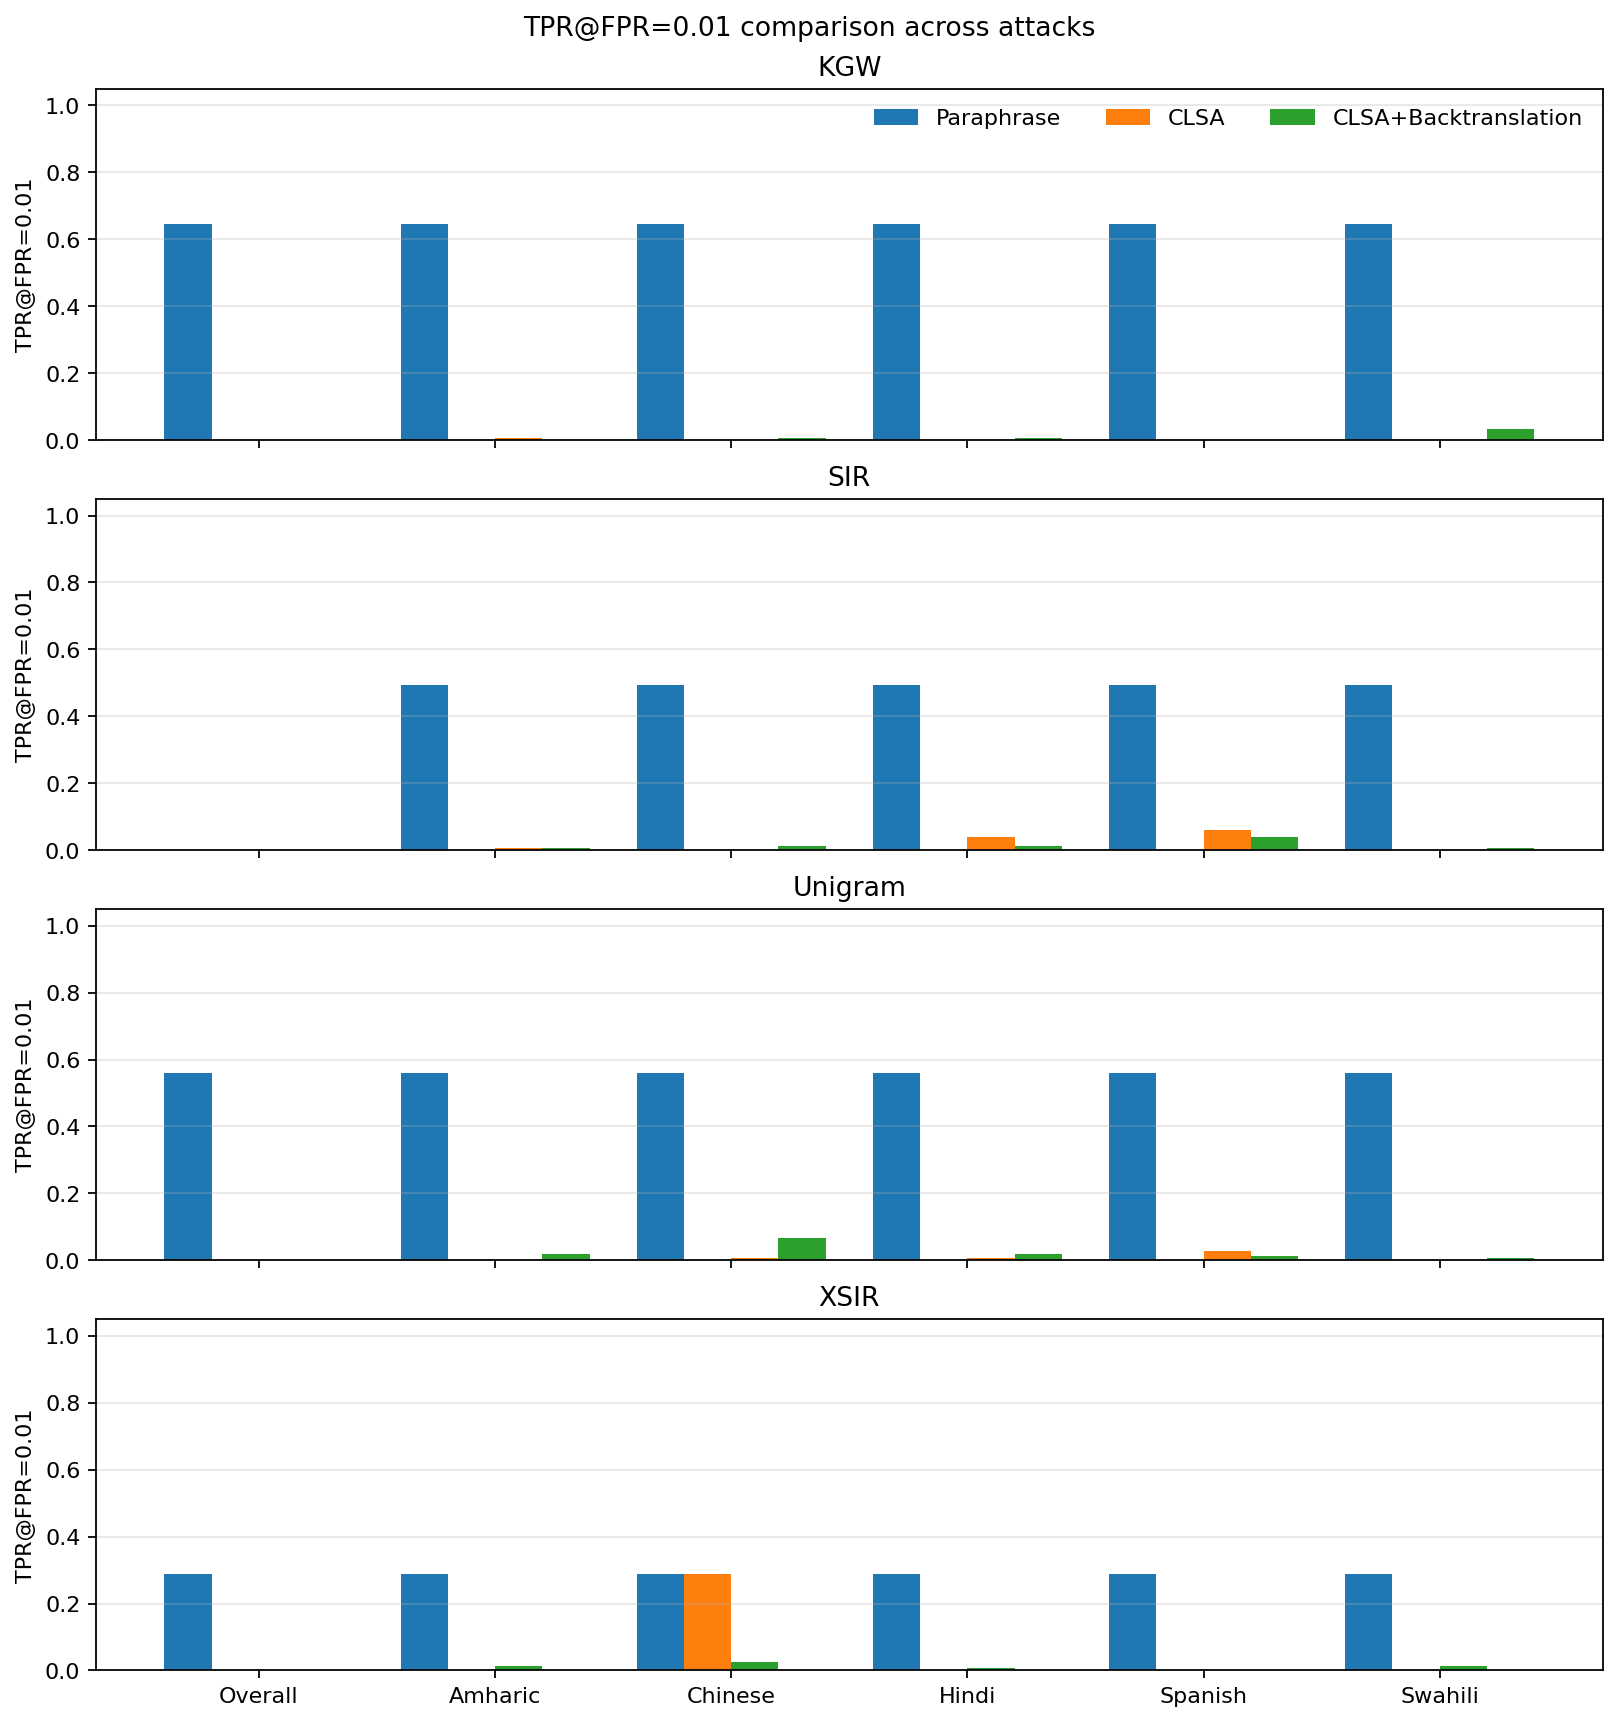
\includegraphics[width=\linewidth]{tpr_fpr_0_01_bars.png}
\caption{TPR at 1\% FPR: CLSA collapses true-positive rates at stringent false-positive operating points.}
\end{figure}
%
\begin{figure}[h]
\centering
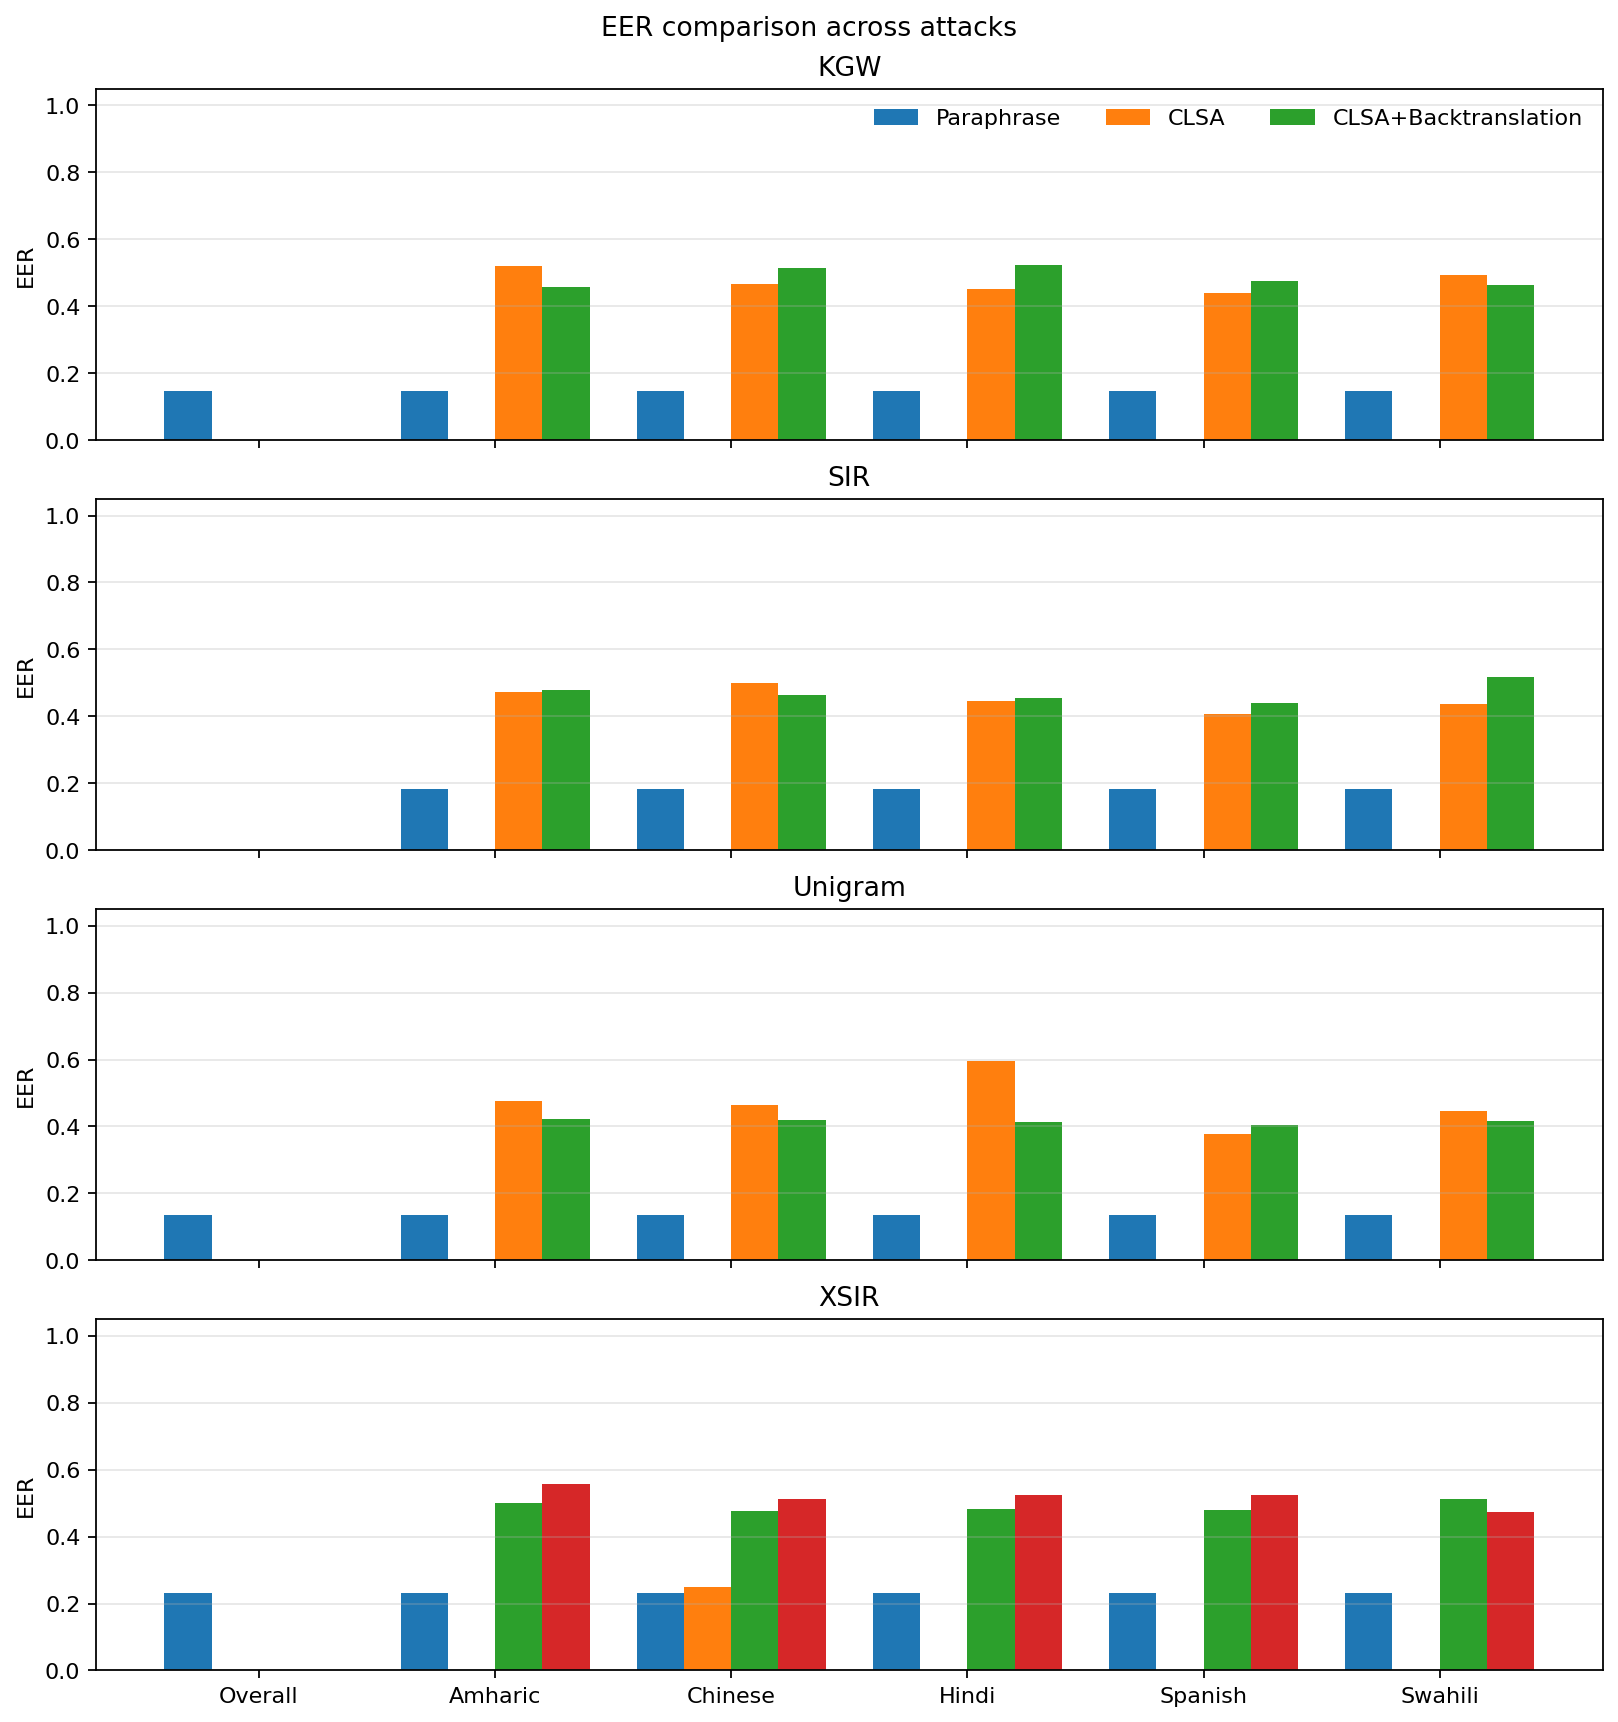
\includegraphics[width=\linewidth]{eer_bars.png}
\caption{Equal Error Rate (EER): higher values under CLSA indicate reduced separability.}
\end{figure}
%
\begin{figure}[h]
\centering
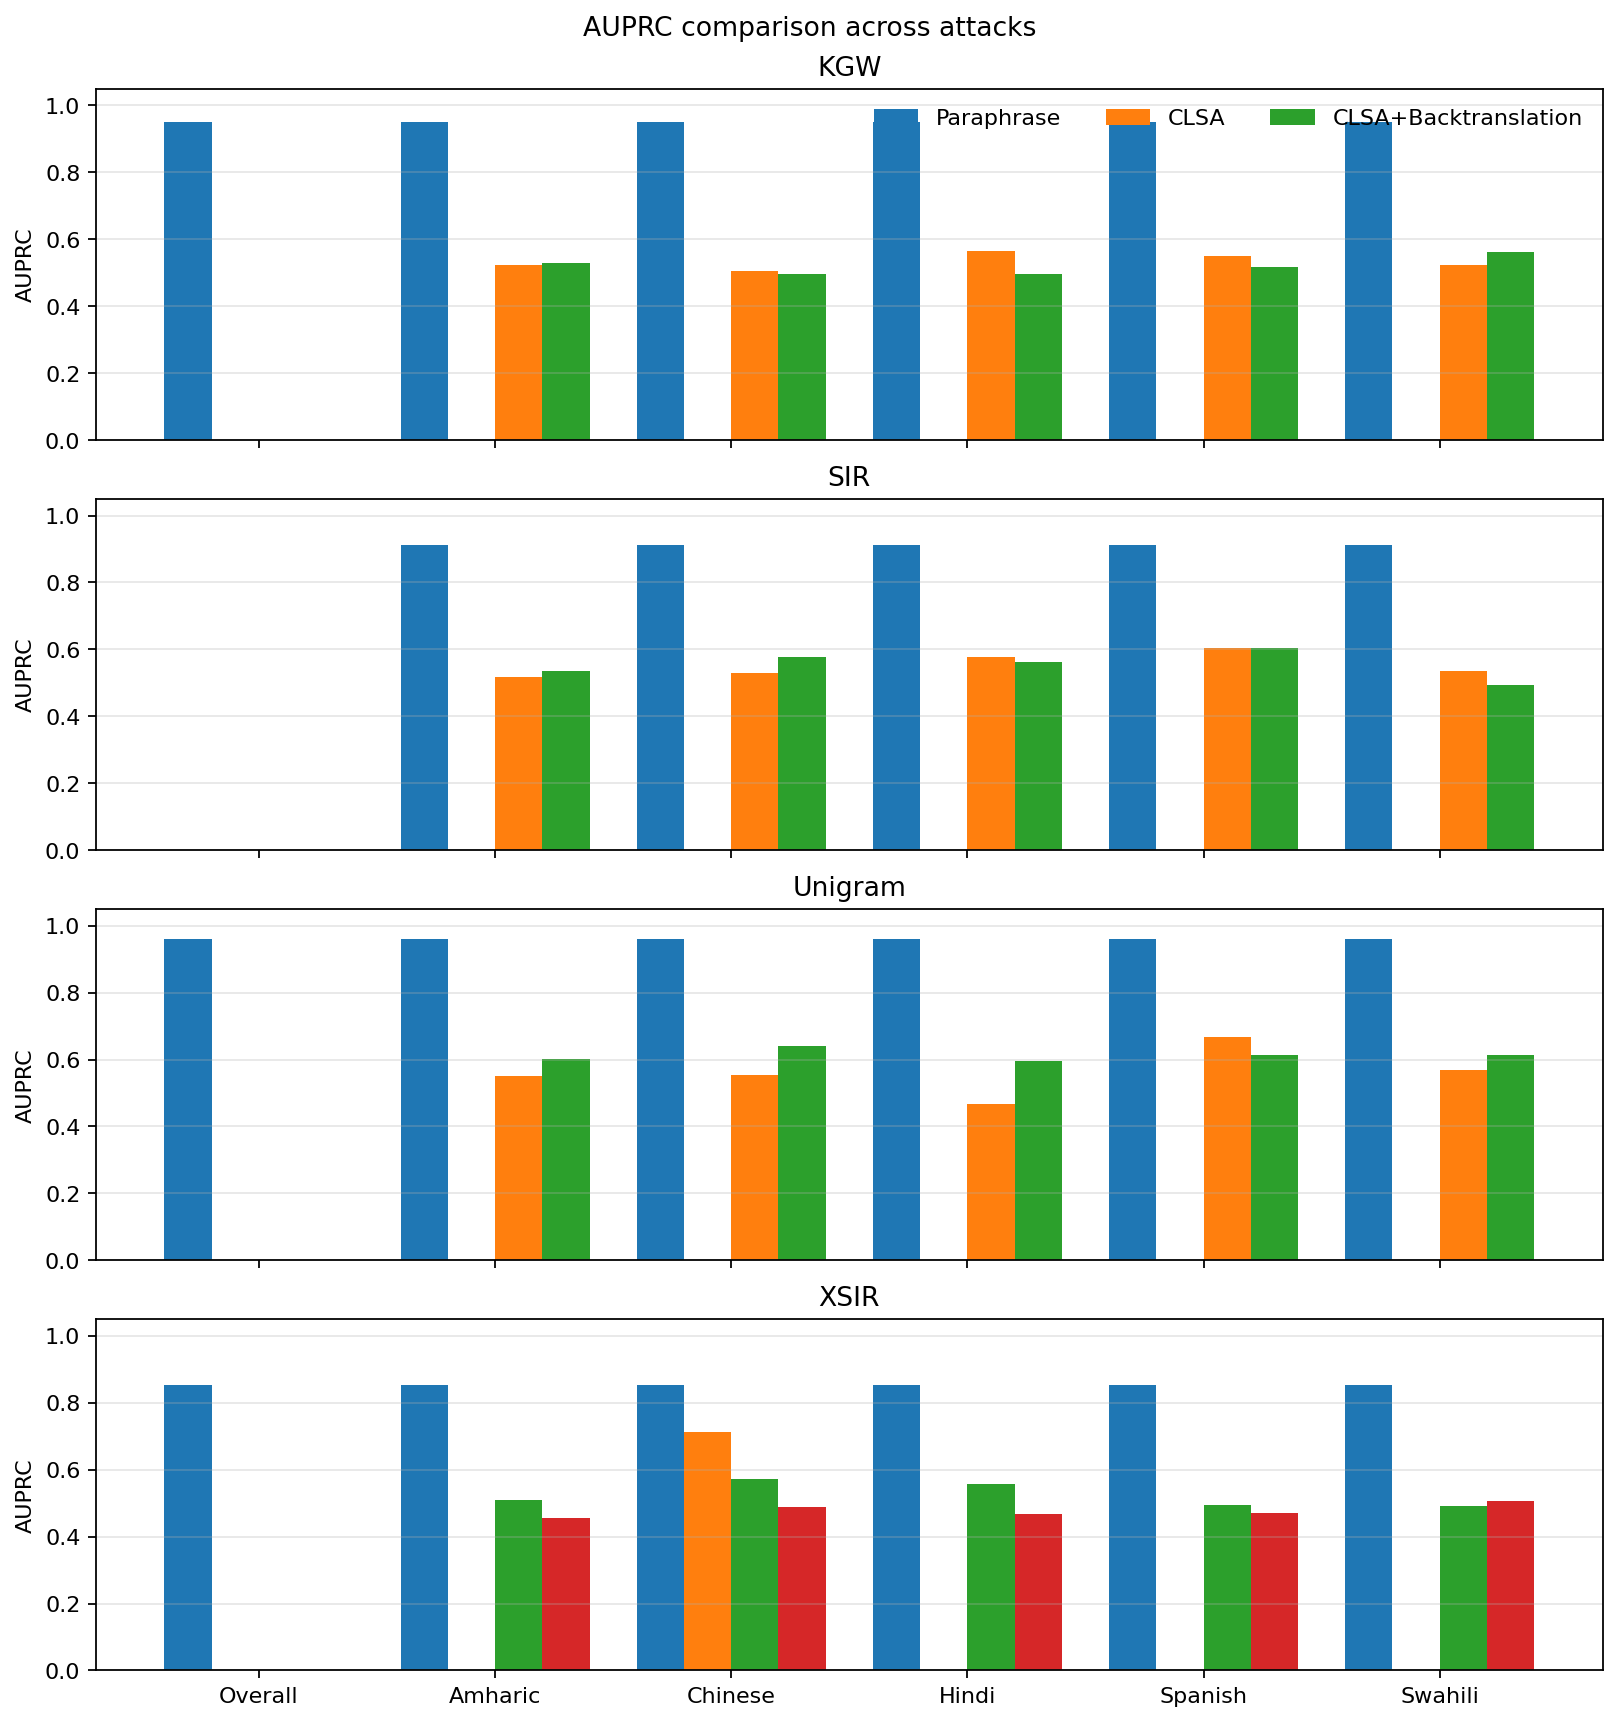
\includegraphics[width=\linewidth]{auprc_bars.png}
\caption{AUPRC by detector and language under baselines vs.\ CLSA.}
\end{figure}
%
\begin{figure}[h]
\centering
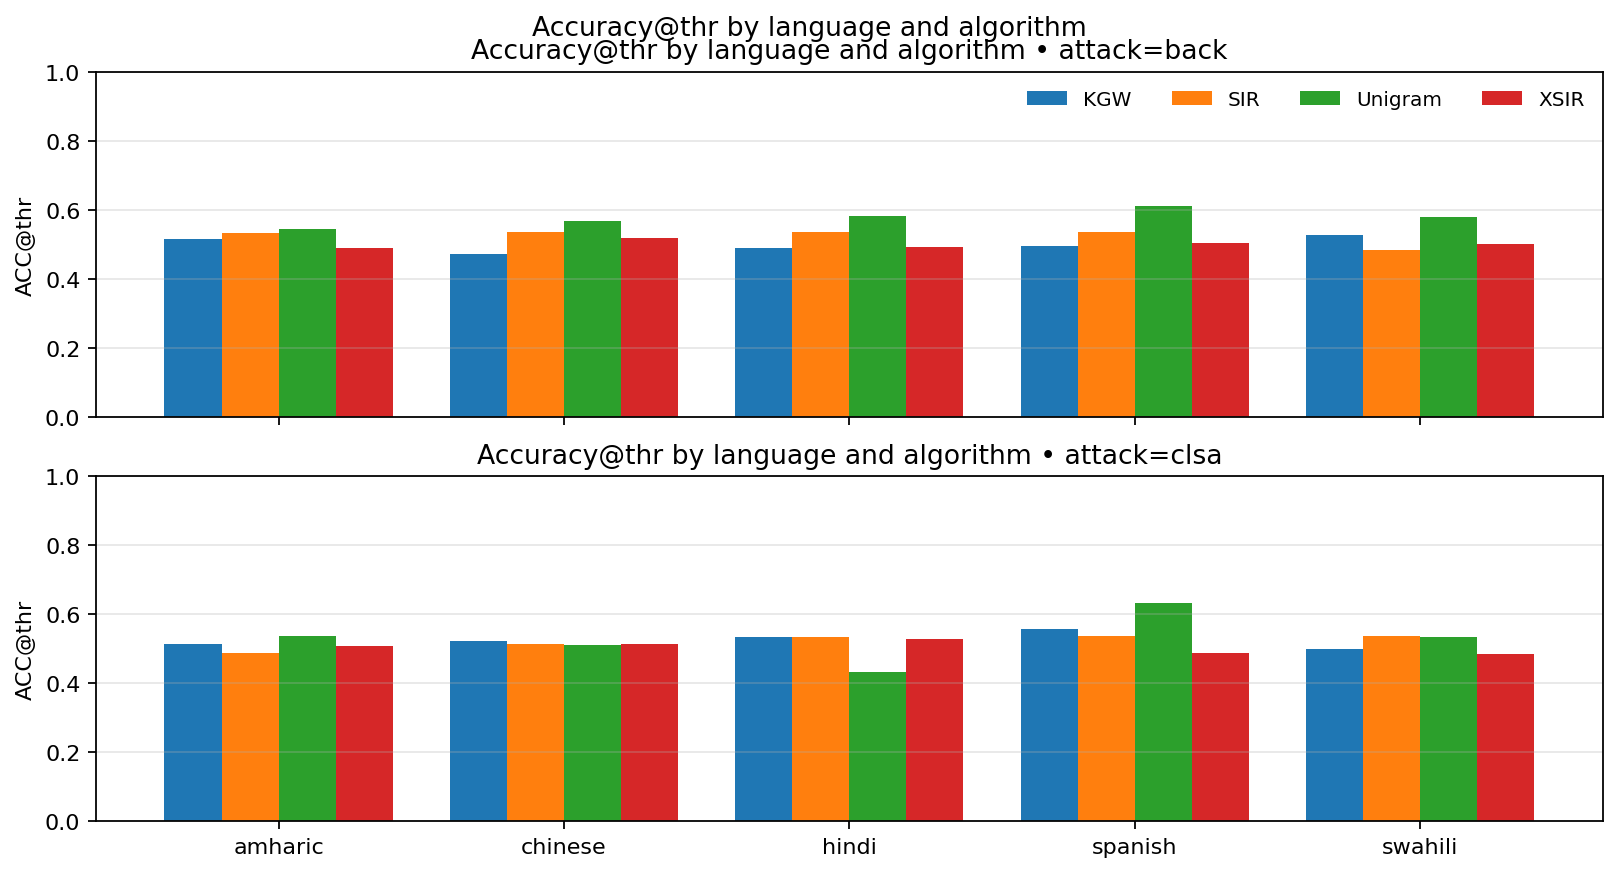
\includegraphics[width=\linewidth]{acc_bars.png}
\caption{Accuracy@thr comparison.}
\end{figure}
%
\begin{figure}[h]
\centering
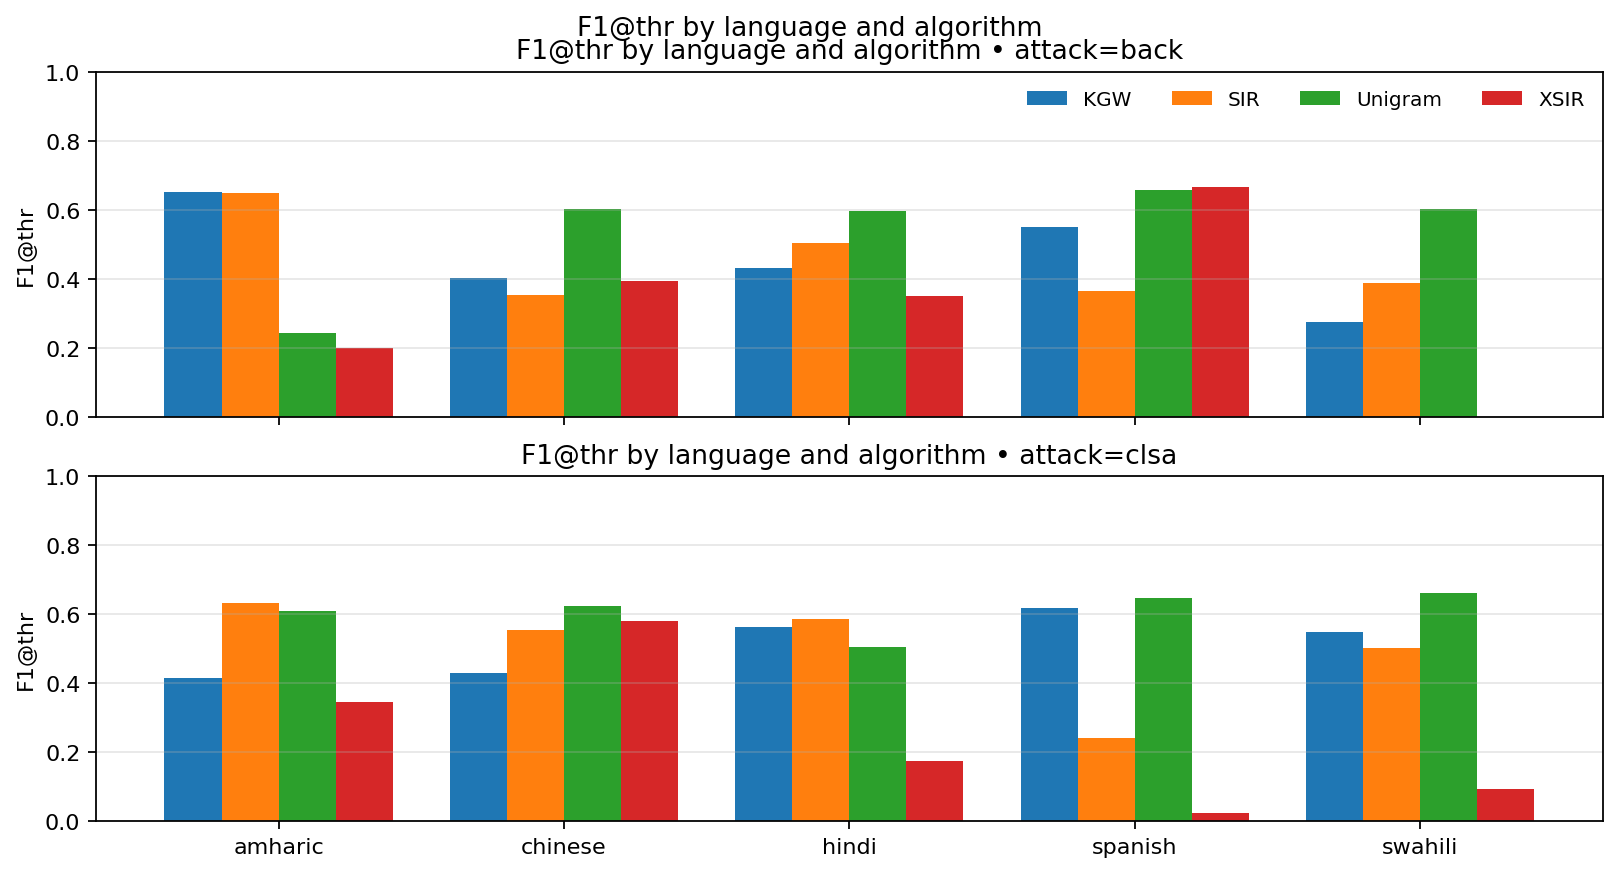
\includegraphics[width=\linewidth]{f1_bars.png}
\caption{F1@thr comparison.}
\end{figure}



\clearpage
% Checklist section
\section*{NeurIPS Paper Checklist}
% \setlength{\parskip}{0pt}

\begin{enumerate}

\item {\bf Claims}
    \item[] Question: Do the main claims made in the abstract and introduction accurately reflect the paper's contributions and scope?
    \item[] Answer: \answerYes{}
    \item[] Justification: The abstract/introduction match the contributions: define CLSA; evaluate KGW/SIR/XSIR/Unigram across five languages with 300/200 splits; analyze why translate→compress erases seeds; and discuss defenses (length‑aware, semantic‑clustered).

\item {\bf Limitations}
    \item[] Question: Does the paper discuss the limitations of the work performed by the authors?
    \item[] Answer: \answerYes{}
    \item[] Justification: §Limitations explicitly covers scope (five languages, four detectors, modest sample sizes), lack of automatic quality metrics, and sensitivity to pivot language and summary budget.

\item {\bf Theory assumptions and proofs}
    \item[] Question: For each theoretical result, does the paper provide the full set of assumptions and a complete (and correct) proof?
    \item[] Answer: \answerNA{}
    \item[] Justification: No new theorems or proofs are introduced; the paper is empirical.

    \item {\bf Experimental result reproducibility}
    \item[] Question: Does the paper fully disclose all the information needed to reproduce the main experimental results of the paper to the extent that it affects the main claims and/or conclusions of the paper (regardless of whether the code and data are provided or not)?
    \item[] Answer: \answerYes{}
    \item[] Justification: We specify detectors, languages, sample counts, models (M2M100, mT5/XLSum), validation‑based thresholds, and report AUROC/AUPRC/EER/TPR@1%FPR; Appendix A enumerates full per‑language tables.


\item {\bf Open access to data and code}
    \item[] Question: Does the paper provide open access to the data and code, with sufficient instructions to faithfully reproduce the main experimental results, as described in supplemental material?
    \item[] Answer: \answerNo{}
    \item[] Justification: To preserve double‑blind review, we do not link code/data in the submission; we plan to release anonymized scripts and tables upon acceptance.


\item {\bf Experimental setting/details}
    \item[] Question: Does the paper specify all the training and test details (e.g., data splits, hyperparameters, how they were chosen, type of optimizer, etc.) necessary to understand the results?
    \item[] Answer: \answerYes{}
    \item[] Justification: §Experimental Setup details detectors, datasets, counts, models, and metrics; thresholds are selected on validation; implementation choices (pivot, budget) are stated.

\item {\bf Experiment statistical significance}
    \item[] Question: Does the paper report error bars suitably and correctly defined or other appropriate information about the statistical significance of the experiments?
    \item[] Answer: \answerNo{}
    \item[] Justification: We report point estimates (AUROC, etc.) without CIs; we will add bootstrap confidence intervals in a camera‑ready.

\item {\bf Experiments compute resources}
    \item[] Question: For each experiment, does the paper provide sufficient information on the computer resources (type of compute workers, memory, time of execution) needed to reproduce the experiments?
    \item[] Answer: \answerNo{}
    \item[] Justification: We did not include detailed compute (GPU/CPU, runtime) in the submission; we will document these in supplemental material.
\item {\bf Code of ethics}
    \item[] Question: Does the research conducted in the paper conform, in every respect, with the NeurIPS Code of Ethics \url{https://neurips.cc/public/EthicsGuidelines}?
    \item[] Answer: \answerYes{}
    \item[] Justification: We follow the NeurIPS Code of Ethics; the paper discusses responsible disclosure and dual‑use considerations in §Broader Impact.


\item {\bf Broader impacts}
    \item[] Question: Does the paper discuss both potential positive societal impacts and negative societal impacts of the work performed?
    \item[] Answer: \answerYes{}
    \item[] Justification: §Broader Impact outlines risks of misuse (watermark removal) and mitigation (defenses, guidance).
\item {\bf Safeguards}
    \item[] Question: Does the paper describe safeguards that have been put in place for responsible release of data or models that have a high risk for misuse (e.g., pretrained language models, image generators, or scraped datasets)?
    \item[] Answer: \answerNA{}
    \item[] Justification: No high‑risk models or datasets are being released.

\item {\bf Licenses for existing assets}
    \item[] Question: Are the creators or original owners of assets (e.g., code, data, models), used in the paper, properly credited and are the license and terms of use explicitly mentioned and properly respected?
    \item[] Answer: \answerYes{}
    \item[] Justification: We cite and respect licenses for M2M100, mT5/XLSum, and any toolkits used (e.g., MarkLLM); license details will be listed in supplemental material.

\item {\bf New assets}
    \item[] Question: Are new assets introduced in the paper well documented and is the documentation provided alongside the assets?
    \item[] Answer: \answerNA{}
    \item[] Justification: We do not introduce new datasets or pretrained models.

\item {\bf Crowdsourcing and research with human subjects}
    \item[] Question: For crowdsourcing experiments and research with human subjects, does the paper include the full text of instructions given to participants and screenshots, if applicable, as well as details about compensation (if any)? 
    \item[] Answer: \answerNA{}
    \item[] Justification: No human subjects or crowdsourcing were involved.

\item {\bf Institutional review board (IRB) approvals or equivalent for research with human subjects}
    \item[] Question: Does the paper describe potential risks incurred by study participants, whether such risks were disclosed to the subjects, and whether Institutional Review Board (IRB) approvals (or an equivalent approval/review based on the requirements of your country or institution) were obtained?
    \item[] Answer: \answerNA{}
    \item[] Justification: Not applicable; no human subjects research.

\item {\bf Declaration of LLM usage}
    \item[] Question: Does the paper describe the usage of LLMs if it is an important, original, or non-standard component of the core methods in this research? Note that if the LLM is used only for writing, editing, or formatting purposes and does not impact the core methodology, scientific rigorousness, or originality of the research, declaration is not required.
    \item[] Answer: \answerYes{}
    \item[] Justification: LLMs are core to the method (watermarked generation, translation via M2M100, summarization via mT5/XLSum, and detector scoring). Their roles and models are described in §Experimental Setup.

\end{enumerate}
\end{document}
